% Diagrama F — quadrante conceitual: desempenho preditivo vs. preservação estrutural.
\documentclass[tikz,border=6pt]{standalone}
% Preâmbulo compartilhado dos diagramas conceituais do relatório CoInfoSim.
% Compilação: xelatex (determinística; nenhum dado experimental é usado).
\usepackage{fontspec}
\setmainfont{Liberation Sans}
\setsansfont{Liberation Sans}
\usepackage{amsmath}
\usepackage{bm}
\usepackage{tikz}
\usetikzlibrary{arrows.meta,positioning,calc,fit,backgrounds,decorations.pathreplacing,matrix,patterns}
\definecolor{CoinAccent}{RGB}{25,80,140}
\definecolor{CoinAccentDark}{RGB}{18,55,95}
\definecolor{CoinAccentPale}{RGB}{237,242,248}
\definecolor{CoinGray}{RGB}{95,95,95}
\definecolor{CoinGrayPale}{RGB}{246,246,246}
\definecolor{CoinWin}{RGB}{76,140,90}    % verde discreto (vitória)
\definecolor{CoinLose}{RGB}{182,88,79}   % vermelho discreto (derrota)
\tikzset{
  bloco/.style={draw=CoinAccentDark, fill=CoinAccentPale, rounded corners=1.2pt,
                align=center, font=\small, inner sep=4pt, minimum height=7mm},
  bloconeutro/.style={draw=CoinGray, fill=CoinGrayPale, rounded corners=1.2pt,
                align=center, font=\small, inner sep=4pt, minimum height=7mm},
  blocoreal/.style={draw=CoinAccentDark, fill=white, rounded corners=1.2pt,
                align=center, font=\small, inner sep=4pt, minimum height=7mm},
  seta/.style={-{Stealth[length=2.4mm]}, thick, CoinAccentDark},
  setacinza/.style={-{Stealth[length=2.4mm]}, thick, CoinGray},
  rotulo/.style={font=\footnotesize\itshape, text=CoinGray, align=center},
}

\begin{document}
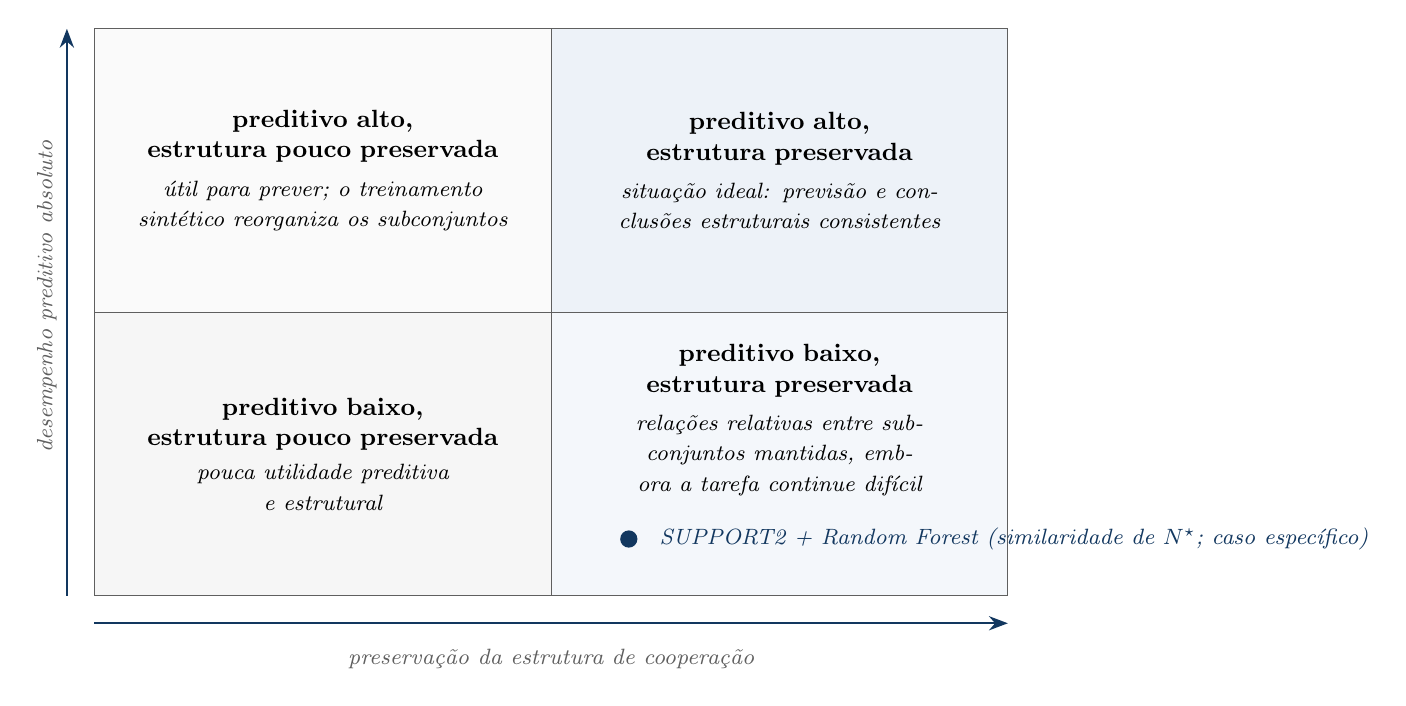
\begin{tikzpicture}
  \def\L{11.6} \def\H{7.2}
  % Quadrantes
  \fill[CoinGrayPale]  (0,0) rectangle (\L/2,\H/2);
  \fill[CoinAccentPale] (\L/2,\H/2) rectangle (\L,\H);
  \fill[CoinGrayPale!60] (0,\H/2) rectangle (\L/2,\H);
  \fill[CoinAccentPale!60] (\L/2,0) rectangle (\L,\H/2);
  \draw[CoinGray] (0,0) rectangle (\L,\H);
  \draw[CoinGray] (\L/2,0) -- (\L/2,\H);
  \draw[CoinGray] (0,\H/2) -- (\L,\H/2);

  % Eixos
  \draw[seta] (-0.35,0) -- (-0.35,\H) node[midway, rotate=90, above=2mm, rotulo] {desempenho preditivo absoluto};
  \draw[seta] (0,-0.35) -- (\L,-0.35) node[midway, below=2mm, rotulo] {preservação da estrutura de cooperação};

  % Conteúdo dos quadrantes
  \node[align=center, font=\small, text width=4.9cm] at (\L*0.25,\H*0.75)
    {\textbf{preditivo alto,\\estrutura pouco preservada}\\[1mm]
     \footnotesize\itshape útil para prever; o treinamento sintético reorganiza os subconjuntos};
  \node[align=center, font=\small, text width=4.9cm] at (\L*0.75,\H*0.75)
    {\textbf{preditivo alto,\\estrutura preservada}\\[1mm]
     \footnotesize\itshape situação ideal: previsão e conclusões estruturais consistentes};
  \node[align=center, font=\small, text width=4.9cm] at (\L*0.25,\H*0.25)
    {\textbf{preditivo baixo,\\estrutura pouco preservada}\\[1mm]
     \footnotesize\itshape pouca utilidade preditiva\\e estrutural};
  \node[align=center, font=\small, text width=4.9cm] at (\L*0.75,\H*0.31)
    {\textbf{preditivo baixo,\\estrutura preservada}\\[1mm]
     \footnotesize\itshape relações relativas entre subconjuntos mantidas, embora a tarefa continue difícil};

  % Marcador do caso SUPPORT2 + Random Forest
  \node[circle, fill=CoinAccentDark, inner sep=2.2pt] (rf) at (\L*0.585,\H*0.10) {};
  \node[rotulo, right=1.5mm of rf, text=CoinAccentDark, align=left]
    {SUPPORT2 + Random Forest (similaridade de $N^{\star}$; caso específico)};
\end{tikzpicture}
\end{document}
